\documentclass[12pt,letterpaper]{article}
\usepackage[utf8]{inputenc}
\usepackage{graphicx} %Para importar gráficos
\usepackage[greek, spanish, mexico]{babel} %Para soportar texto en griego con el comando \greektext y que el contenido del documento esté en español de México
\usepackage[hidelinks]{hyperref} %Para el enlace al final del documento

\title{El número $\Pi$}
\author{Eduardo René Rodríguez Ávila}
\parskip=0.3cm
\begin{document}

  \maketitle

\section{Introducción}

$\Pi$ (pi) es la relación entre la longitud de una circunferencia y su diámetro (ver figura 1), en geometría euclidiana. Es un número irracional y una de las constantes matemáticas más importantes. Se emplea frecuentemente en matemáticas, física e ingeniería. 

\begin{figure}[h] 
\centering
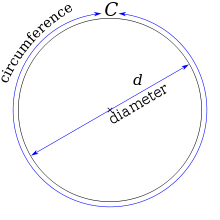
\includegraphics[width=0.4\textwidth]{img/circ_sobre_diam.png}
\caption{$\Pi$ es obtenido por la relación $\frac{C}{d}  = \pi$}
\end{figure}

El valor numérico de $\Pi$, truncado a sus primeras cifras, es el siguiente:

\begin{displaymath}
  \pi  \approx  3.14159265358979323846 \cdots
\end{displaymath}

El valor de $\Pi$ se ha obtenido con diversas aproximaciones a lo largo de la historia, siendo una de las constantes matemáticas que más aparece en las ecuaciones de la física, junto con el número e. Cabe destacar que el co\-ciente entre la longitud de cualquier circunferencia y la de su diámetro no es constante en geometrías no euclídeas.

\section{El nombre $\Pi$}

La notación con la letra griega $\Pi$ proviene de la inicial de las palabras de origen griego ``\textgreek{περιφέρεια}'' (periferia) y ``\textgreek{περίμετρον}'' (perímetro) de una círcunferencia, notación que fue utilizada primero por William Oughtred (1574-1660), y propuesto su uso por el matemático galés William Jones (1675-1749), aunque fue el matemático Leonhard Euler, con su obra ``Introducción al cálculo infinitesimal'' de 1748, quien la popularizó. Fue conocida an\-te\-rior\-men\-te como constante de Ludolph (en honor al matemático Ludolph van Ceulen) o como constante de Arquímedes (que no se debe confundir con el número de Arquímedes).

\begin{figure}[h] 
	\centering
	\includegraphics[width=0.2\textwidth]{img/pi.png}
	\caption{Letra griega $\pi$. Símbolo adoptado en 1706 por William Jones y popularizado por Leonhard Euler.}
\end{figure}

\section{Historia del cálculo del valor $\Pi$}

El matemático griego Arquímedes (siglo III a. C.) fue capaz de de\-ter\-mi\-nar el valor de $\Pi$, entre el intervalo comprendido por $3 \frac{10}{71}$, como valor mínimo, y $3 \frac{1}{7}$, como valor máximo. Con esta aproximación de Arquímedes se obtiene un valor con un error que oscila entre 0.024\% y 0.040\% sobre el valor real. El método usado por Arquímedes era muy simple y consistía en cir\-cuns\-cri\-bir e inscribir polígonos regulares de n-lados en circunferencias y calcular el perímetro de dichos polígonos. Arquímedes empezó con hexágonos circunscritos e inscritos, y fue doblando el número de lados hasta llegar a polígonos de 96 lados.

\begin{figure}[h] 
	\centering
	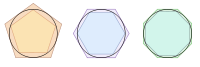
\includegraphics[width=0.7\textwidth]{img/Archimedes_pi.png}
	\caption{Método de Arquímedes para encontrar dos valores que se aproximen al número $\Pi$, por exceso y defecto.}
\end{figure}


Alrededor del año 20 d. C., el arquitecto e ingeniero romano Vitruvio calcula $\Pi$ como el valor fraccionario 25/8 midiendo la distancia recorrida en una revolución por una rueda de diámetro conocido.

En el siglo II, Claudio Ptolomeo proporciona un valor fraccionario por aproximaciones:

\begin{displaymath}
	\pi \approx \frac{377}{120} = 3.1416 \cdots
\end{displaymath}

Mas información en: \url{http://es.wikipedia.org/wiki/N\%C3\%BAmero\_\%CF\%80}
\end{document}